%
%
\subsection{MATLAB: Filterdesign}\label{subsec:digifilt:fda:exercises}
%
%

\paragraph{Aufgabe 1: Entwurf von FIR-Filtern mit der Fenstermethode}

\begin{enumerate}
	\item Generieren sie einen Bandpass mit beliebigem Toleranzschema mit Hilfe der Fenstermethode. Welche Unterschiede fallen ihnen bei Verwendung unterschiedlicher Fenster auf. Dokumentieren sie die Ergebnisse, indem sie von jedem Filter einen Ausdruck anfertigen. Welche Grenzfrequenzen verwenden sie f�r ihr Filter?
	Speichern sie ihre erzeugten Fenster und Filter im folgenden Verzeichnis: \pathtomatlab{Empf�nger\textbackslash MATLAB\_Filterdesign\textbackslash Aufgabe\_01}
	\answergame{2}{Die entsprechenden Graphiken finden sie in der MATLAB-Musterl�sung im Verzeichnis \pathtomatlab{Empf�nger\textbackslash MATLAB\_Filterdesign\textbackslash Aufgabe\_01} }
	\vspace{0.5cm}
	\ifthenelse{\printsolution}{
		\\Die Musterl�sung wurde mit den in Abb. \ref{fig:A1_01} eingestellten Parametern erstellt
		\begin{figure}[ht]
		\centering 
		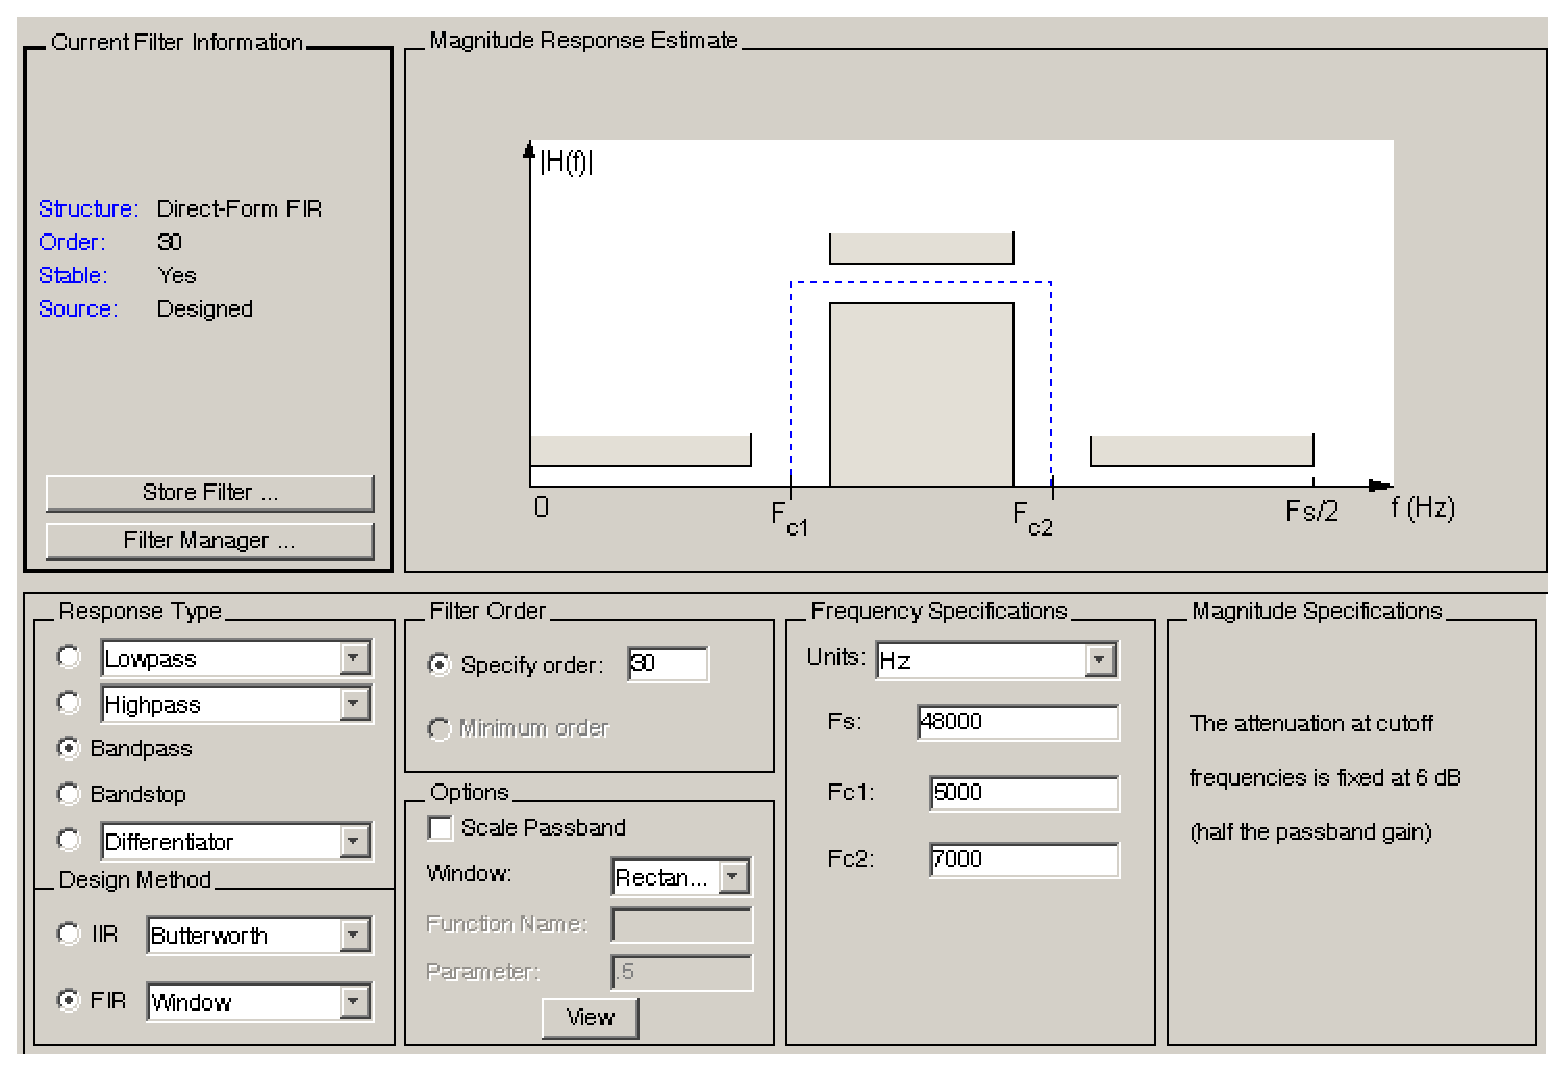
\includegraphics[width=12cm]{bilder/empfaenger/filterdesign/BPWinPar}
		\caption{Eingestellte Parameter}
		\label{fig:A1_01}
		\end{figure}
		
		Die Abb. \ref{fig:A1_02} und \ref{fig:A1_03} stellen das verwendete Rechteck-Fenster und den 						resultierenden Ampitudenverlauf des Filters dar.
		\begin{figure}[ht]
			\centering
			\begin{minipage}[c]{.41\linewidth}
				\centering 
				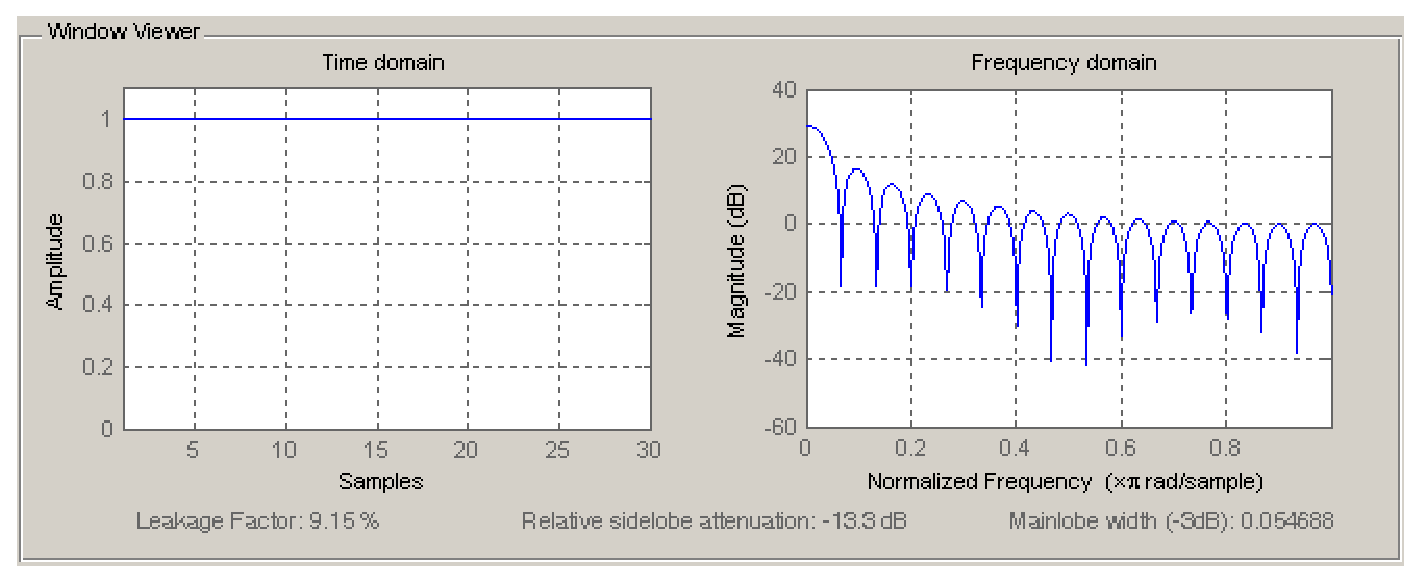
\includegraphics[width=8cm]{bilder/empfaenger/filterdesign/Rechteckfenster}
				\caption{Rechteckfenster}
				\label{fig:A1_02}
			\end{minipage}
			\begin{minipage}[c]{.10\linewidth}
				\hfill
			\end{minipage}
			\begin{minipage}[c]{.41\linewidth}
				\centering 
				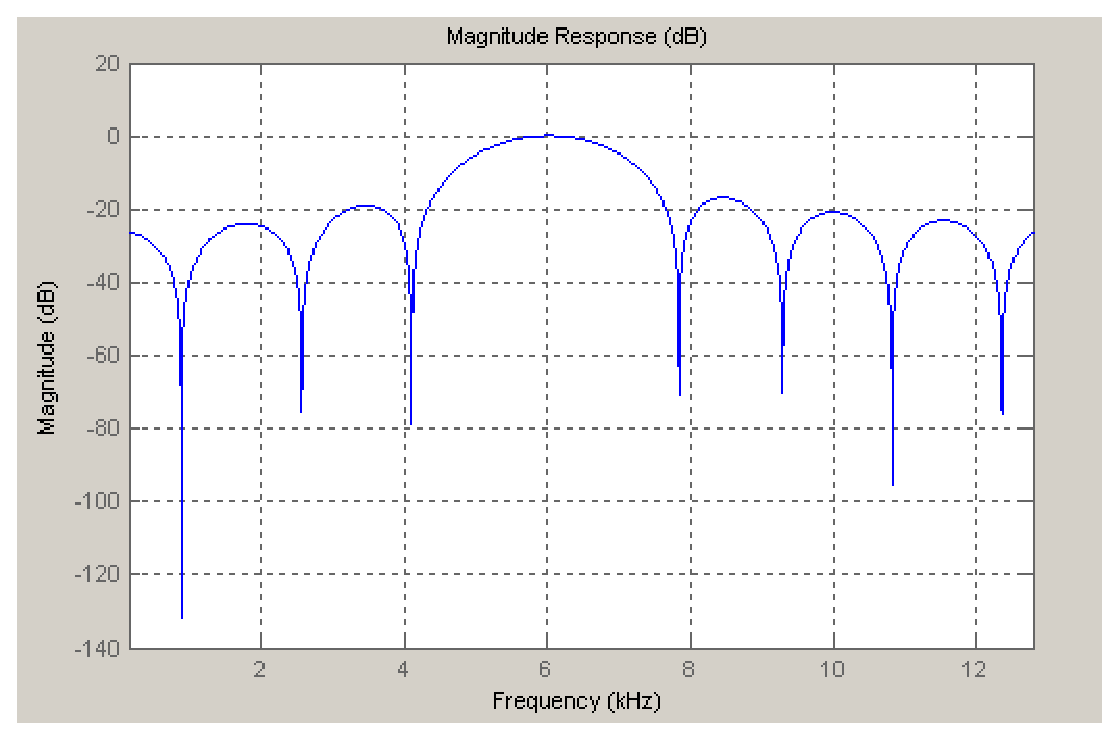
\includegraphics[width=7cm]{bilder/empfaenger/filterdesign/BPWinRect}
				\caption{Frequenzgang mit Rechteckfenster}
				\label{fig:A1_03}
			\end{minipage}
		\end{figure}

		Jetzt das Ganze nochmal mit einem Hanning-Fenster (Abb. \ref{fig:A1_04} und \ref{fig:A1_05})
		
			\begin{figure}[ht]
			\centering
			\begin{minipage}[c]{.41\linewidth}
				\centering 
				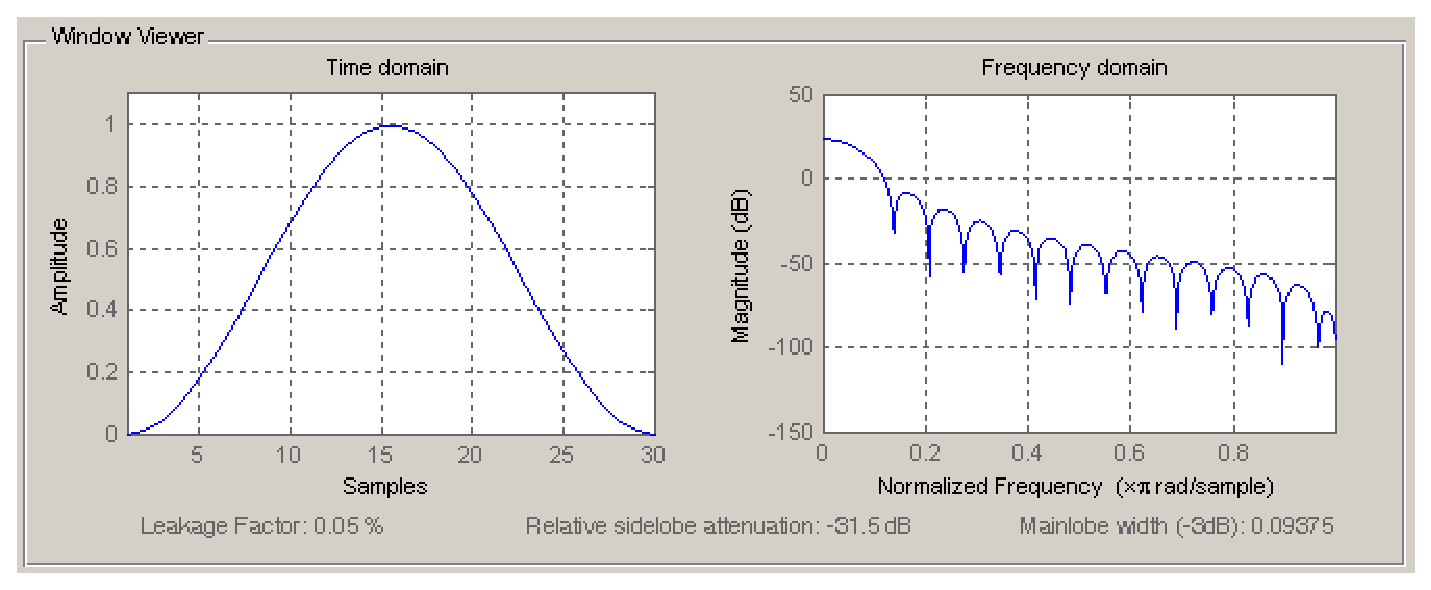
\includegraphics[width=8cm]{bilder/empfaenger/filterdesign/Hanning}
				\caption{Hanningfenster}
				\label{fig:A1_04}
			\end{minipage}
			\begin{minipage}[c]{.10\linewidth}
				\hfill
			\end{minipage}
			\begin{minipage}[c]{.41\linewidth}
				\centering 
				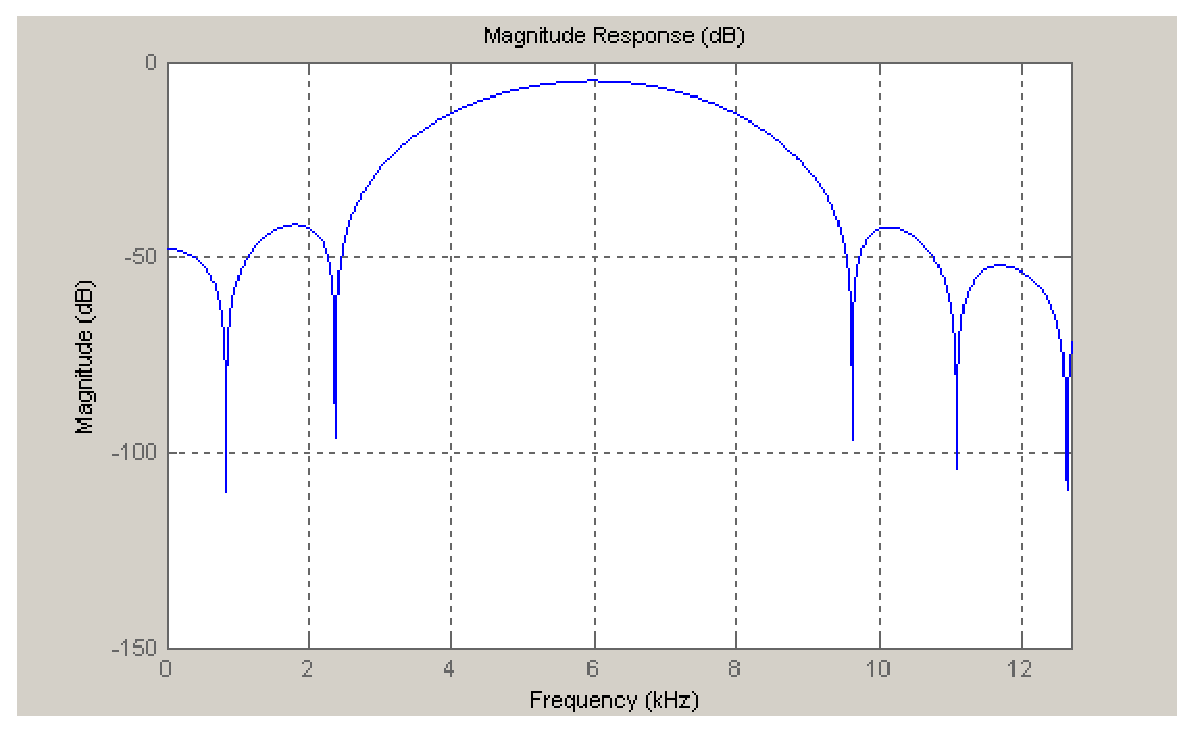
\includegraphics[width=7cm]{bilder/empfaenger/filterdesign/BPWinHann}
				\caption{Frequenzgang mit Hanningfenster}
				\label{fig:A1_05}
			\end{minipage}
		\end{figure}
		
		Zum Abschluss noch mit dem Kaiserfenster (Parameter Beta: 1.8; Abb. \ref{fig:A1_06} und 								\ref{fig:A1_07})
		
		\begin{figure}[ht]
		\centering
			\begin{minipage}[c]{.41\linewidth}
				\centering 
				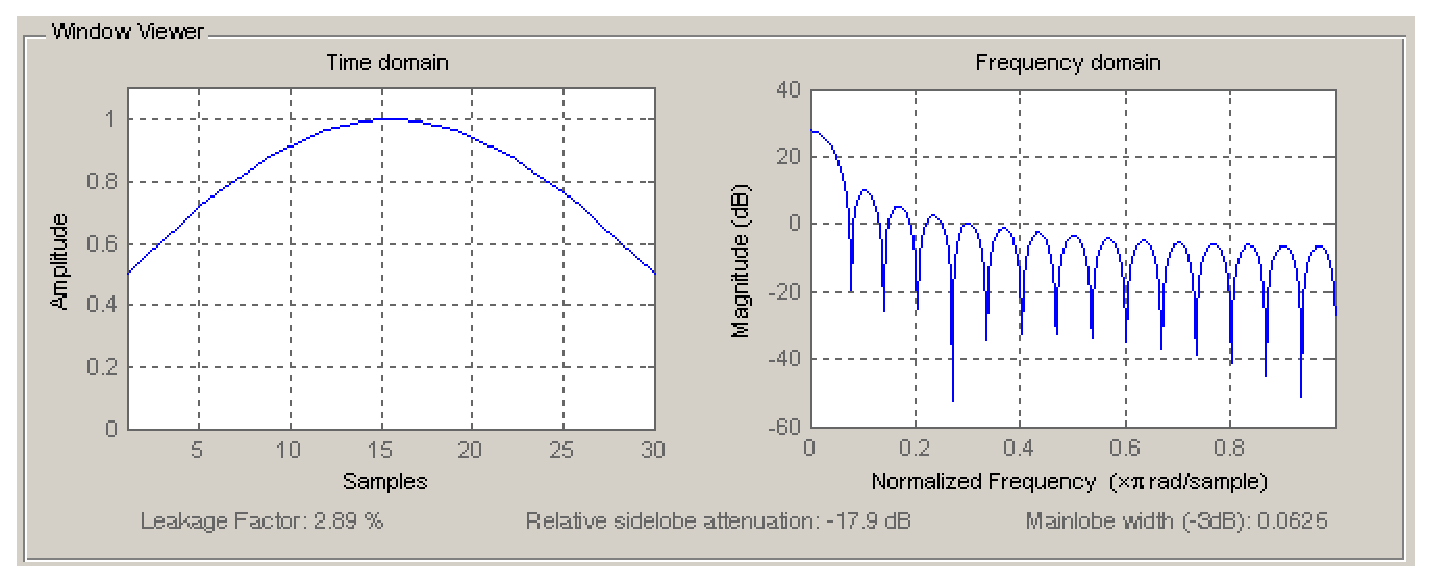
\includegraphics[width=8cm]{bilder/empfaenger/filterdesign/Kaiserfenster}
				\caption{Kaiserfenster, Beta: 1.8}
				\label{fig:A1_06}
			\end{minipage}
			\begin{minipage}[c]{.10\linewidth}
				\hfill
			\end{minipage}
			\begin{minipage}[c]{.41\linewidth}
				\centering 
				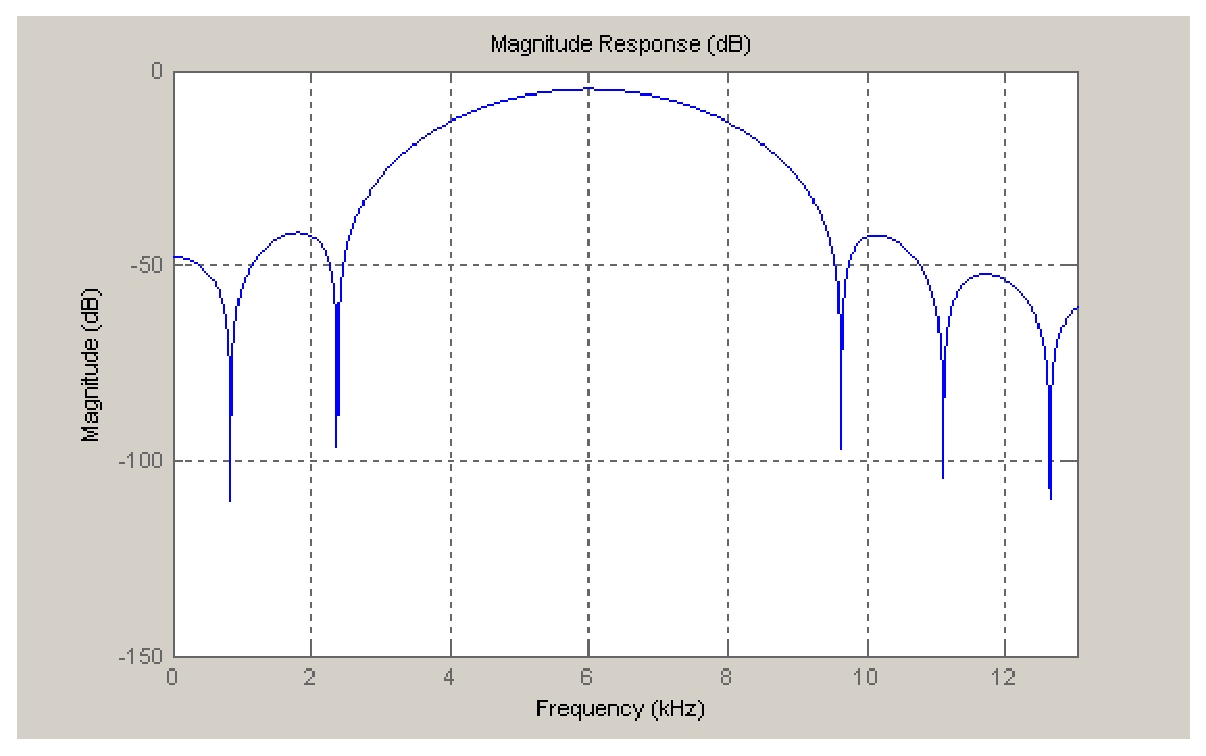
\includegraphics[width=7cm]{bilder/empfaenger/filterdesign/BPWinKaiser}
				\caption{Frequenzgang mit Kaiserfenster}
				\label{fig:A1_07}
			\end{minipage}
		\end{figure}
		}
	\item Wie unterscheiden sich die einzelnen Amplitudenfrequenzg�nge voneinander? Welchen w�rden sie bevorzugen?
		\answergame{6}{Die Nebenliniend�mpfung von Hanning und Kaiser-Fenster ist deutlich besser, als beim Rechteckfenster. Daf�r ist der effektive Durchlassbereich beim Rechteckfenster schmaler, es besitzt steilere Flanken.}
		
\end{enumerate}

\paragraph{Aufgabe 2: Optimalmethode}
\begin{enumerate}
		\item Entwerfen sie nun einen Bandpass mit der Optimalmethode. Wie unterscheidet sich das Ergebnis von den Ergebnissen der Fenstermethode? Speichern sie ihren entworfenen Bandpass im Verzeichnis \pathtomatlab{Empf�nger\textbackslash MATLAB\_Filterdesign\textbackslash Aufgabe\_02} ab.
			\answergame{3}{Einen Musterentwurf finden sie in \pathtomatlab{Empf�nger\textbackslash MATLAB\_Filterdesign\textbackslash Aufgabe\_02} In den Abb. \ref{fig:A2_01} und \ref{fig:A2_02} sind die entworfenen Filter inklusive der verwendeten Parameter dargestellt.}
			\vspace{0.5cm}
			\ifthenelse{\printsolution}{
				
				\begin{figure}[ht]
					\centering 
					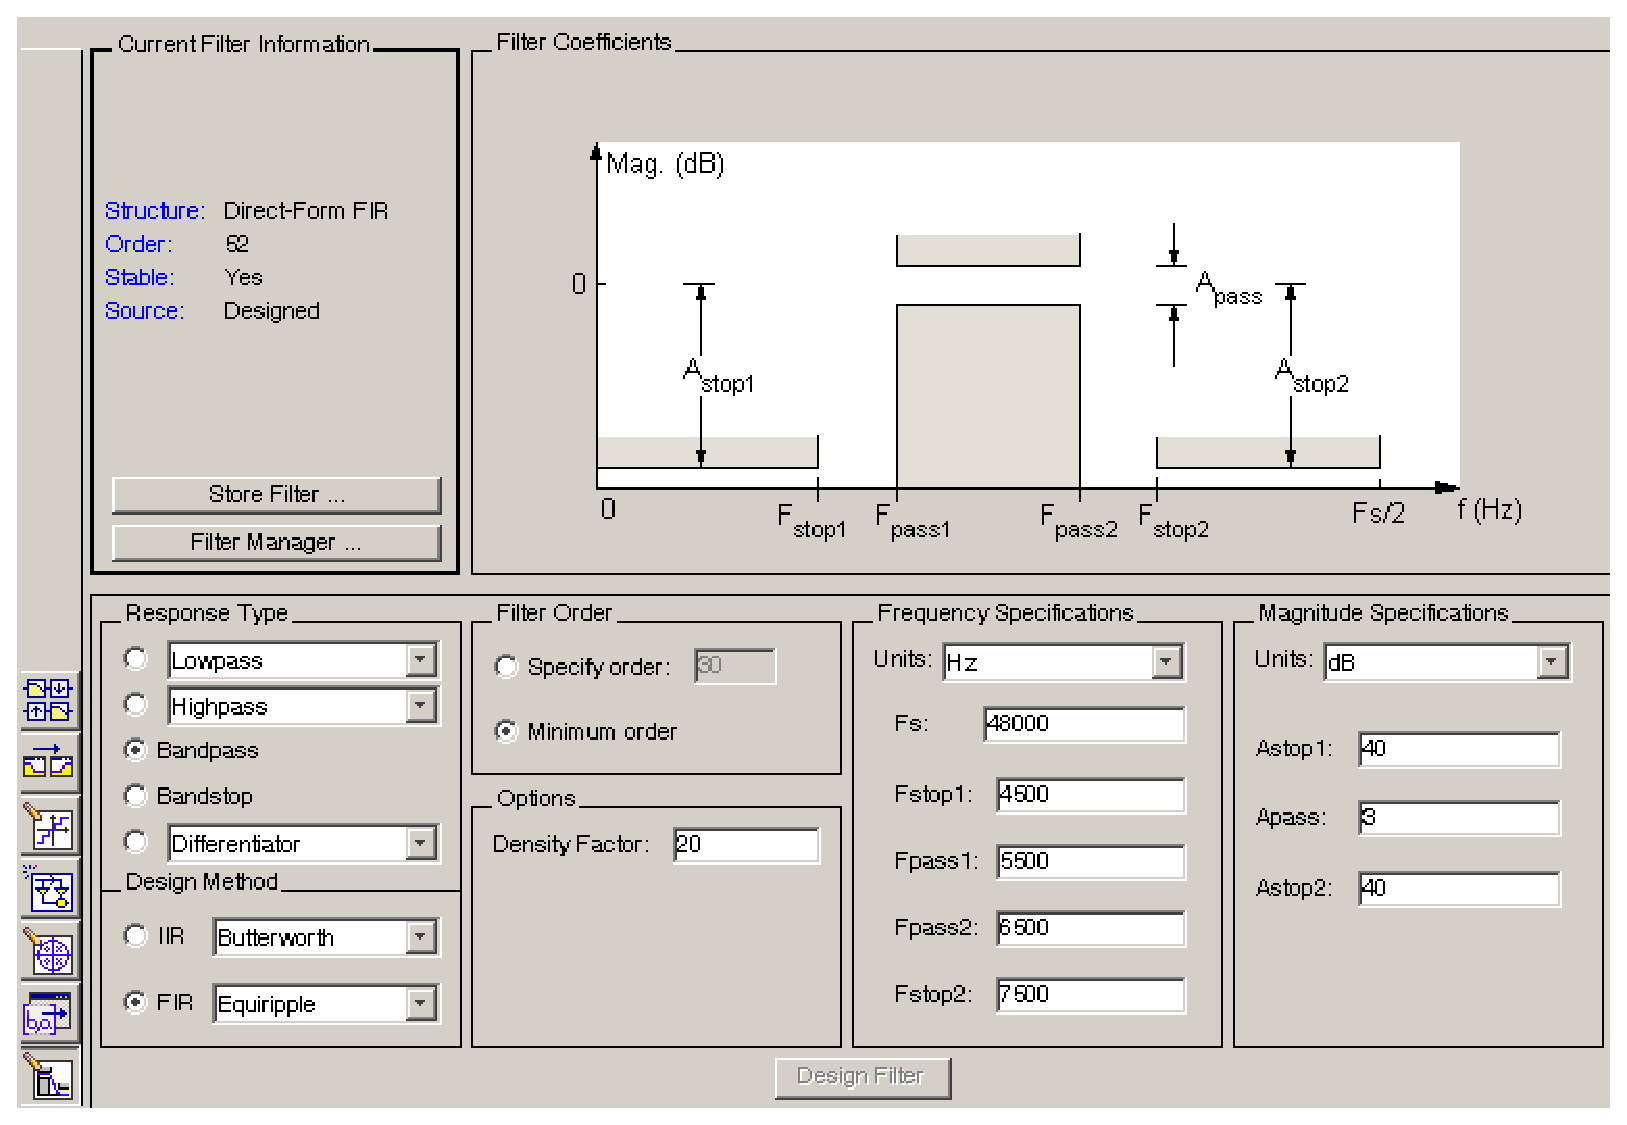
\includegraphics[width=12cm]{bilder/empfaenger/filterdesign/BPOptPar}
					\caption{Bandpass-Design mit der Optimalmethode - Parameter}
					\label{fig:A2_01}
				\end{figure}
				\begin{figure}[ht]
					\centering 
					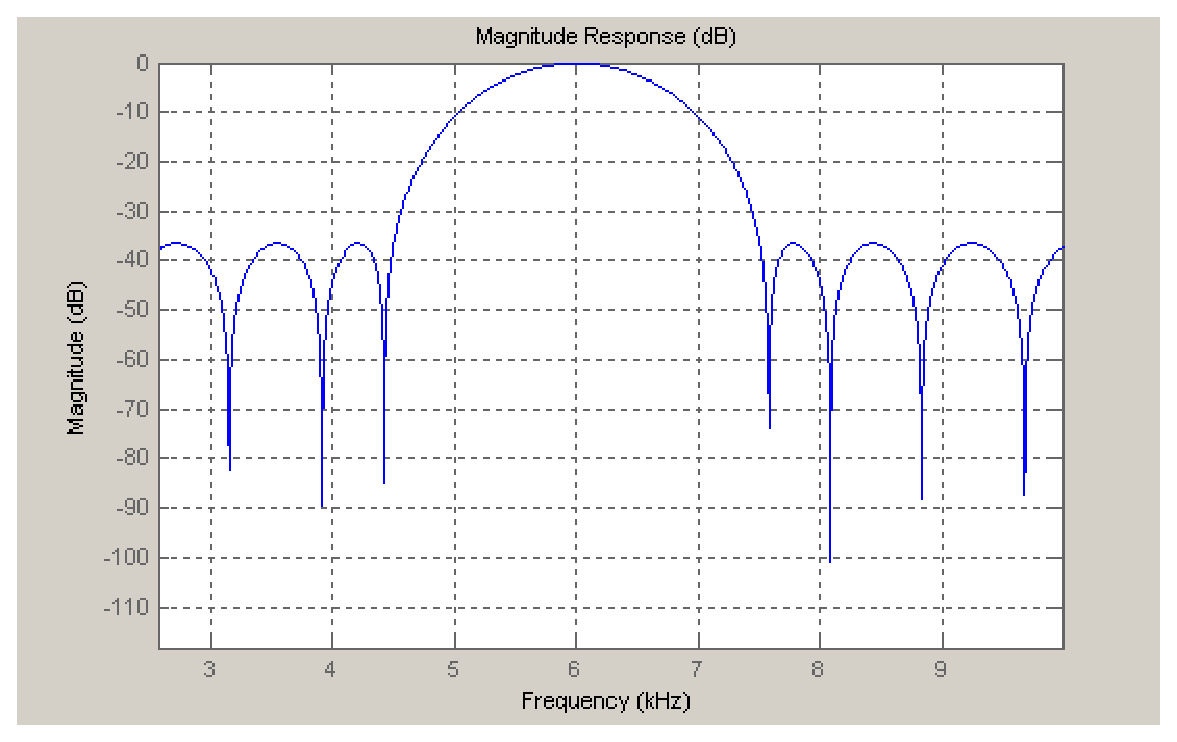
\includegraphics[width=6cm]{bilder/empfaenger/filterdesign/BPOpt}
					\caption{Bandpass-Design mit der Optimalmethode}
					\label{fig:A2_02}
				\end{figure}
			}
				
	\item Gehen sie zu quantisierten Filterkoeffizienten mit 8 Bit Wortl�nge �ber. Vergleichen sie die Amplitudenfrequenzg�nge der Filter. 
			\answergame{3}{Wie erwartet kommt es durch die reduzierte Genauigkeit der Koeffizienten zu einer sichtbaren Verschlechterung des Betragsfrequenzgangs (vgl. Abb. \ref{fig:A2_03}). Auch hier wieder die Musterentw�rfe im Verzeichnis \pathtomatlab{Empf�nger\textbackslash MATLAB\_Filterdesign\textbackslash Aufgabe\_02}}
			\ifthenelse{\printsolution}
			{
				\begin{figure}[ht]	
					\centering 
					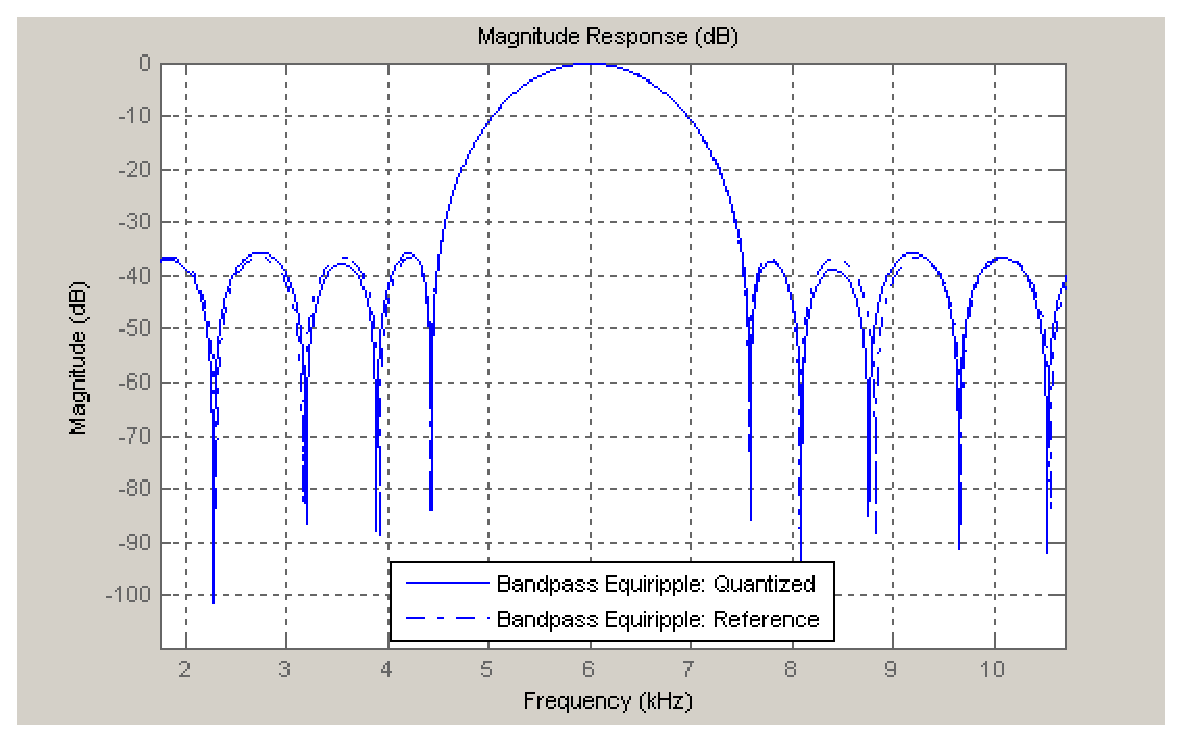
\includegraphics[width=8cm]{bilder/empfaenger/filterdesign/BPOptQuant} 
					\caption{Bandpass-Design mit der Optimalmethode und quantisierten Koeffizienten} 
					\label{fig:A2_03} 
				\end{figure}
			}
			
\end{enumerate}

\paragraph{Aufgabe 3: Portierung nach MATLAB und Testen des Filters}
\begin{enumerate}	
		
		\item Exportieren sie ihren Filter nun in den MATLAB-Workspace. 
		
		\item Machen sie sich mit der Filterfunktion \textit{filtfir\_symm\_qa.m} im Verzeichnis \pathtomatlab{Empf�nger\textbackslash MATLAB\_Filterdesign\textbackslash Aufgabe\_03} vertraut.
		
		\item Erzeugen sie mit ihrem in Versuch 5 aufgebauten Modulator ein beliebiges FSK Signal und wenden sie den entworfenen Filter darauf an. Funktioniert ihr Design? 
		\answergame{1}{JA! Eine m�gliche L�sung finden sie im Verzeichnis \pathtomatlab{Empf�nger\textbackslash MATLAB\_Filterdesign\textbackslash Aufgabe\_03} im MATLAB-Skript \textit{A3.m}}
		
		Was sehen sie? 
		\answergame{3}{Im Idealfall sollte nur die Frequenz, die sich im Durchlassbereich des Bandpasses befindet vom Filter durchgelassen werden. Alle anderen Anteile des Signals werden unterdr�ckt.}
		
		Ein Tipp: um etwas sehen zu k�nnen sollte eine der beiden FSK-Frequenzen im Durchlassbereich des Bandpasses liegen!
		
\end{enumerate}
